\section{Modifizierte Baugruppen}

\color{blue}
Im Zuge des Umbaus mussten Anpassungen an einigen Baugruppen vorgenommen werden. Dabei wurde immer grossen Wert darauf gelegt, möglichst wenig vom Originalzustand abzuweichen. Die durchgeführten Anpassungen werden in diesem Kapitel erläutert.

\subsection{Originaler Hauptschalter} \label{orig_HS}
Der originale Hauptschalter des \textsc{Detroit}s befindet sich unter der Sitzbank auf der Fahrerseite und besteht aus einem Hebel, der einen Kupferkontakt zwischen zwei Schienenstücke drückt. Dieser Hebel ist mechanisch mit der Standbremse gekoppelt, sodass bei betätigter Standbremse kein Stromkreis geschlossen werden kann.

Dieser Schaltmechanismus ist leider nicht mehr voll funktionsfähig, da der Hebel nicht mehr genügend Kraft ausüben kann, um einen sauberen Kontakt zu gewähren (die Standbremse funktioniert jedoch weiterhin mit voller Kraft). Auch mit einem Nachspannen der Feder konnte die Kraft nicht genügend erhöht werden, um einen sauberen Kontakt sicher herzustellen.

Da im Zuge des Umbaus sowieso ein moderner gasisolierter Hauptschalter eingebaut wurde, ist der originale Hauptschalter im Grunde genommen überflüssig. Er könnte also theoretisch ausgebaut und überbrückt werden. Es wurde aber bewusst entschieden, das Originalteil im Fahrzeug angeschlossen zu lassen. Um trotzdem die elektrische Verbindung zwischen den beiden Kontakten zu gewähren, wurde innerhalb des Gehäuses des alten Schalters eine Kupferbrücke zwischen den beiden Anschlussstellen hergestellt, wie Abbildung \ref{fig:Bruecke_HS} zeigt:

\begin{figure}[h!]
\begin{minipage}{0.49\textwidth}
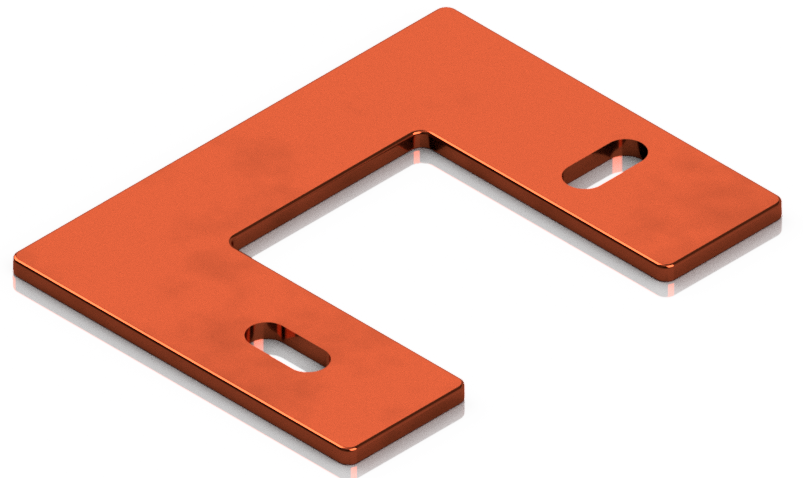
\includegraphics[width=\textwidth]{images/Bruecke_HS.png}
\end{minipage}\begin{minipage}{0.49\textwidth}
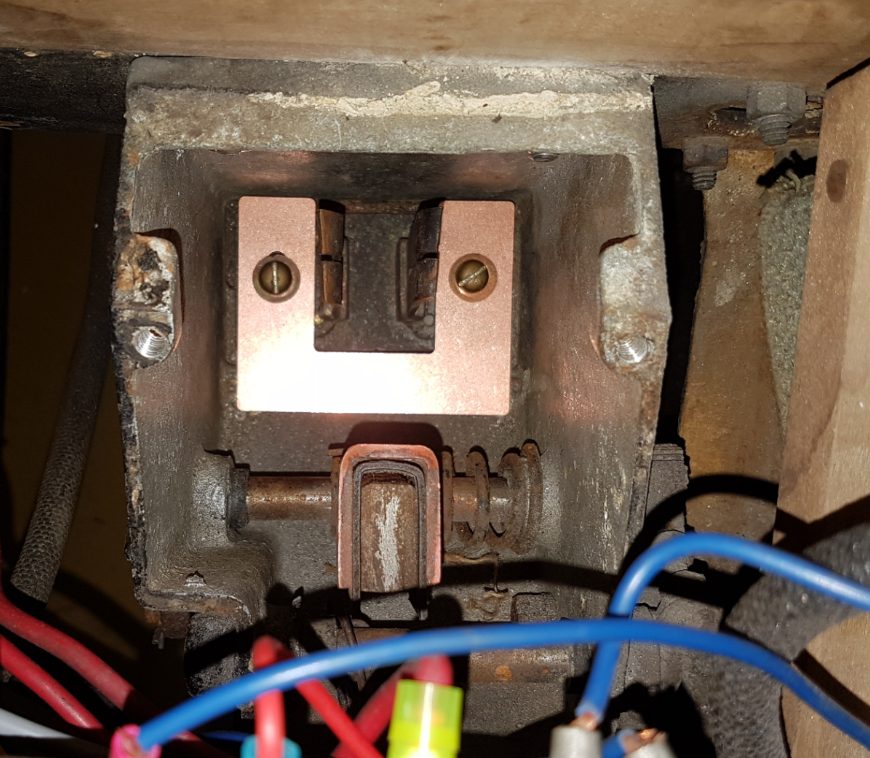
\includegraphics[width=\textwidth]{images/U-Profil.png}
\end{minipage}
\caption{\textcolor{blue}{Die Kupferbrücke als CAD-Zeichnung (links) sowie eingebaut im originalen Hauptschaltergehäuse}}%
\label{fig:Bruecke_HS}%
\end{figure}

Mit dieser Kupferbrücke konnten die Kontaktprobleme des originalen Hauptschalters behoben werden.


\subsection{Shunt}
Ein Shunt ist ein definierter Widerstand, über dem die Spannung gemessen wird, und daraus auf den Strom zurück geschlossen werden kann. Auch im \textsc{Detroit} war ein solcher Shunt zur Strommessung eingebaut. Bei einem früheren Umbau des Fahrzeuges wurden einige Gewinde aufgebohrt, sodass am Ende mehrere unterschiedliche Grössen vorhanden waren. Im Zuge des aktuellen Umbaus sollten diese vereinheitlicht werden. Unglücklicherweise wurde dabei der Shunt beschädigt, welcher aufgrund der benötigten Genauigkeit als Messglied nicht repariert werden kann. Aus diesem Grund wurde ein neuer Shunt angefertigt.

Um den Widerstandswert des Shunts zu erhalten, muss die Empfindlichkeit des Anzeigegerätes bekannt sein. Aus diesem Grund wurde ein Abgleich mit der Skalenanzeige durchgeführt, was zu folgendem Ergebnis führte:
\begin{equation*}\begin{aligned}
	100\text{ A}\ &\rightarrow\ 75.3\text{ mV}\\
	50\text{ A}\ &\rightarrow\ 37.8\text{ mV}
\end{aligned}\end{equation*}
Wie man sieht, passen die Werte sehr gut zusammen. Damit lässt sich nun ein Widerstandswert für den Shunt bestimmen, wie Formel \ref{eq:rshunt} zeigt:

\begin{equation}
R_{Shunt}=\frac{U}{I}=\frac{75.3\text{ mV}}{100\text{ A}}\approx\quad\underline{0.75\text{ m}\Omega}
\label{eq:rshunt}
\end{equation}

Zusammen mit diesem Widerstandswert lässt sich die maximale Abwärme des Shunts bestimmen. Dabei wird als Maximalstrom $150$ A angenommen, wie es auf dem alten Shunt eingeprägt war. Formel \ref{eq:shunt_pv} zeigt die Berechnung der Verlustleistung für den maximalen Strom sowie einen angenommenen durchschnittlichen Strom von $80$ A:

\begin{equation}\begin{aligned}
	P_{v,max}&=I_{max}^2\cdot R_{Shunt}=\left(150\text{ A}\right)^2\cdot0.75\text{ m}\Omega=\quad\underline{16.9\text{ W}}\\[6pt]
	P_{v,nom}&=I_{nom}^2\cdot R_{Shunt}=\left(80\text{ A}\right)^2\cdot0.75\text{ m}\Omega=\quad\underline{4.8 \text{ W}}
\label{eq:shunt_pv}
\end{aligned}\end{equation}

Daraus resultieren einige Anforderungen an den Shunt bzw. das Material, aus welchem er gefertigt ist: \begin{itemize}
	\item Der Werkstoff muss temperaturbeständig sein, insbesondere sollte keine Korrosion oder physikalische Veränderung bei erhöhter Temperatur auftreten.
	\item Die Verlustwärme muss abgeführt werden können. Es sollte also eine Bauform mit grosser Oberfläche gewählt werden.
	\item Um einen stabilen Shunt bauen zu können, sollte die Querschnittsfläche gross sein, was einen hohen spezifischen Widerstand erfordert.
	\item Der Werkstoff muss -- um die gewünschte Form herstellen zu können -- gut bearbeitbar sein.
	\item Die Anschlussblöcke sollten vom Widerstandswert her irrelevant sein gegenüber dem Shunt, weswegen sie massiv aus Kupfer vorzusehen sind.
	\item Die Genauigkeit sollte gross genug sein, um die analoge Anzeige nicht zu verschlechtern, dazu kann eine Genauigkeit von $10$ \% gefordert werden. Auch die Änderung durch Temperaturerhöhung sollte in diesem Bereich liegen.
\end{itemize}

Aufgrund der genannten Bedingungen wurde ein rostfreier Stahl 1.4301 \cite{4301} gewählt. Dieser Werkstoff ist sehr robust, sowohl mechanisch als auch chemisch, hat einen hohen spezifischen Widerstand von $0.73\ \frac{\Omega \cdot \text{mm}^2}{\text{m}}$ und ist als Stahl gut bearbeitbar. Die Länge des Widerstandselementes wird beinahe beibehalten. Es wird eine ursprüngliche Länge von 2 Zoll ($50.8$ mm) vermutet. Die Länge des neuen Shunts beträgt $50$ mm. Damit kann die benötigte Querschnittsfläche bestimmt werden, gezeigt in Formel \ref{eq:shunt_a}:

\begin{equation}
	A_{Shunt}=\frac{\rho\cdot l_{Shunt}}{R_{Shunt}}=\frac{0.73\ \frac{\Omega\cdot\text{mm}^2}{\text{m}}\cdot 0.05\text{ m}}{0.75\text{ m}\Omega}=\quad\underline{48.67\text{ mm}^2}
\label{eq:shunt_a}
\end{equation}

Mit diesem Sollwert für den Querschnitt wurde ein Shuntelement und ein kompletter Widerstand erstellt. Für die Bauteile befinden sich die 2D-Ableitungen im Anhang unter \ref{app:2d}. Folgend soll Abbildung \ref{fig:shunt} noch den fertigen Shunt zeigen, wie er im CAD erstellt wurde:

\begin{figure}[h!]
\begin{minipage}{0.49\textwidth}
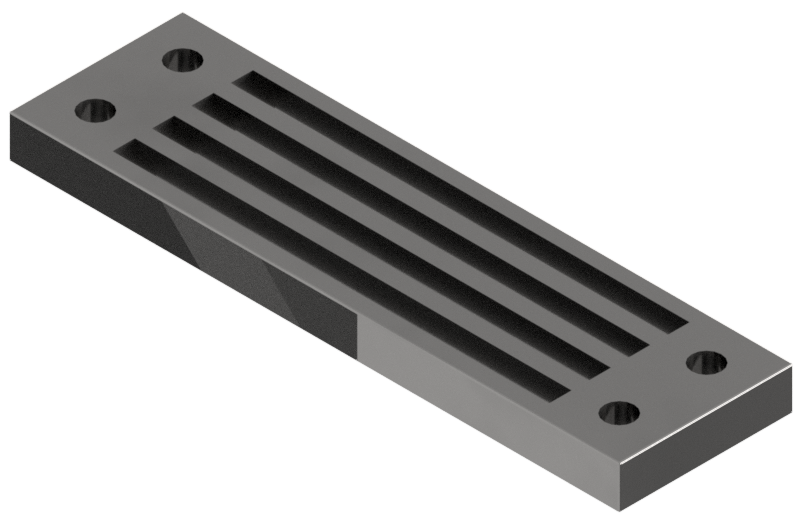
\includegraphics[width=\textwidth]{images/Shunt.png}
\end{minipage}\begin{minipage}{0.49\textwidth}
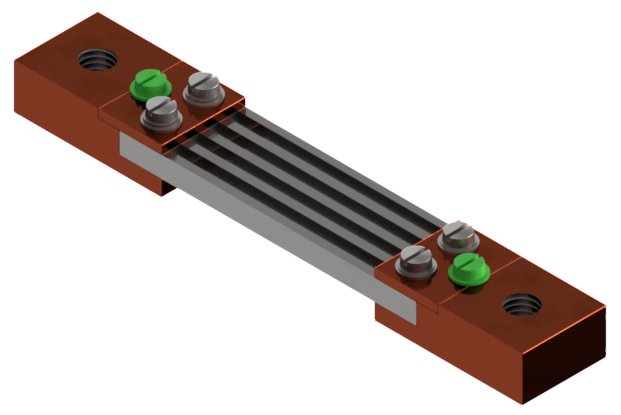
\includegraphics[width=\textwidth]{images/Shunt_komplett.png}
\end{minipage}
\caption{\textcolor{blue}{Das Widerstandselement alleine (links) beziehungsweise mit den Montageblöcken aus Kupfer (rechts). Die grüne Schraubverbindung dient dem Abgreifen der Spannung am Shunt}}%
\label{fig:shunt}%
\end{figure}

\subsection{Verkabelung}
Für die neuen Batterien, welche sich beide im Heck befinden, mussten neue Starkstromleitungen verlegt werden. Prinzipiell wurde aber nur neu verlegt, was nicht aus der bestehenden Verkabelung übernommen werden konnte. Konnte auf die bestehenden Leitungen zurück gegriffen werden, so wurden diese benutzt. Konkret wurden die Leitungen zur ursprünglich vorne platzierten Batterie vom Stufenschalter her nach Hinten neu verlegt, sowie der "`Zwischenabgriff"' für den neuen Hauptschalter, welcher sich zwischen Stufenschalter und Shunt befindet und deswegen vom gesamten Strom durchflossen wird. Alle anderen Leitungen des Antriebsstranges mussten nicht angepasst werden.

Um einen Ansatz für die Dimensionierung zu haben, wurde auf die Niederspannungsinstallationsnorm (NIN) von 2010 \cite{NIN} zurückgegriffen. Diese ist zwar für Hausinstallationen gedacht, wobei dabei die selben Probleme wie z.B. Erwärmung von Leitungen auftreten. Dabei wurde die Referenz-Verlegeart \textit{B2 Kabel in Rohr auf Holzwand} gewählt, da die Leitungen in Rohren und an einigen Stellen auf Holz verlegt sind, was den ungünstigsten Fall darstellt. Die Batterien sind mit $100$ A abgesichert, wobei die beiden unabhängigen Batterien zwei unabhängige Stromkreise bilden. Dieses Verfahren, welches auch für die anderen Starkstromleitungen angewandt wurde, ist für die Batterieleitungen exemplarisch im Anhang unter \ref{app:nin} gezeigt. Folglich wurden die Leitungen mit diesem Querschnitt gewählt. Als weiterer Vergleich können die originalen Leitungen herangezogen werden, welche minim dünner sind, womit der gewählte Querschnitt sicherlich ausreichend ist.

Das selbe Vorgehen wurde für die Ladekabel durchgeführt. Hier beträgt der Ladestrom während der Konstantstrom-Ladephase $19.7$ A, die Norm schreibt für $20$ A einen Querschnitt von $2.5$ mm$^2$ vor. Die Tests haben allerdings eine starke Erwärmung der Leitung gezeigt, weswegen hier mit $4$ mm$^2$ ein grösserer Querschnitt gewählt wurde. Diese beiden Leitungen führen von der Front mit den Ladegeräten zum Heck mit den Batterien.

Die Schwachstromverkabelung beinhaltet hauptsächlich die Kommunikationsleitungen zwischen Batterie im Heck und Steuerung in der Frontklappe. Hier wurde auf ein Telefonkabel vom Typ U72 2x4x0.8 \cite{u72} zurück gegriffen. Dieses Kabel hat die benötigte Aderzahl, weitere kritische Anforderungen waren nicht gestellt. Auch diese Leitung wurde zum Schutz in einem Kunststoffrohr verlegt.

Die $12$ V-Verkabelung wurde teils erneuert und teils so belassen, wie sie ursprünglich war. Zentraler Knotenpunkt ist das hundertjährige Sicherungsbrett, gezeigt in Abbildung \ref{fig:Sicherungsbrett}.

Eingespeist wird das $12$ V-Netz durch ein $2.5$ mm$^2$ Kabel direkt vom DC/DC-Wandler, der sich in der Steuerungsbox befindet und das ganze $12$ V-Netz versorgt. Ebenfalls wird mit dem selben Kabel der Not-Aus-Schalter eingeschlauft, der im Notfall das gesamte Fahrzeug (inklusive Beleuchtung) spannungslos machen kann. Damit wird auch die (lediglich elektrisch) verriegelte Abstellung des \textsc{Detroit}s ermöglicht. Dieser Not-Aus-Schalter befindet sich in der Fahrerkabine unterhalb der Sitzbank. Die Verkabelung der Hupe, Vorderlichter, Meterlicht (Beleuchtung des Volt- und Amperemeters) und Innenbeleuchtung wurde auf dem alten Stand belassen. Die Blinkerschaltung erhält ein neues Kabel 5x$1$ mm$^2$ vom Sicherungsbrett resp. Blinkrelais und musste an der Seitenwand zum Drehschalter geführt werden. Beim Kabel zu den Blinkern handelt es sich um ein 3x$1$ mm$^2$ wobei die Adernfarben braun und blau jeweils rechts und links bedeuten und grün-gelb dem Rückleiter entspricht. Diese beiden Kabel sind vom Typ $TD$ und werden ansonsten im $230$ VAC-Netz verwendet. Für das Rücklicht, was ein Stand- und ein Bremslicht beinhaltet, wurde ein 3x$0.75$ mm$^2$ Kabel verwendet. Zusätzlich wurde ebenfalls ein 2x$0.75$ mm$^2$ verwendet um den Endschalter mit dem Bremslicht zu verbinden.

\color{black}